\subsection{Find patient age from XRay}
\label{sec:warmup4}

    We were given chest X-ray images of patients using which we have to fine-tune a model to determine the age of patients.

\subsubsection{Dataset}
    The provided dataset have $80$ training x-ray images and $165$ testing images. As there was no validtion set, I have randomly splited the training dataset into validation and training set in ration 1:9 respictively. The images in this dataset were color image with shape $2048 \times 2048$, which is resized to image of size $224 \times 224$.

\subsubsection{Training}

    This is a regression problem, thus a few changes is required to the model used in classifying gender of patients. The last Log Softmax layer is not required, thus eliminated from the model graph as shown in \cref{fig:age_model}. The model is trained using mean ssquare error function with Adam optimizer having a learning rate of $0.003$. Additionally, in this experiment too, early stopping with a patience of 3 epochs is implemented to halt the model training. \Cref{fig:gender-learning-curve} illustrates the learning curve of the training and validation sets.

    \begin{figure}[htbp]
        \centering
        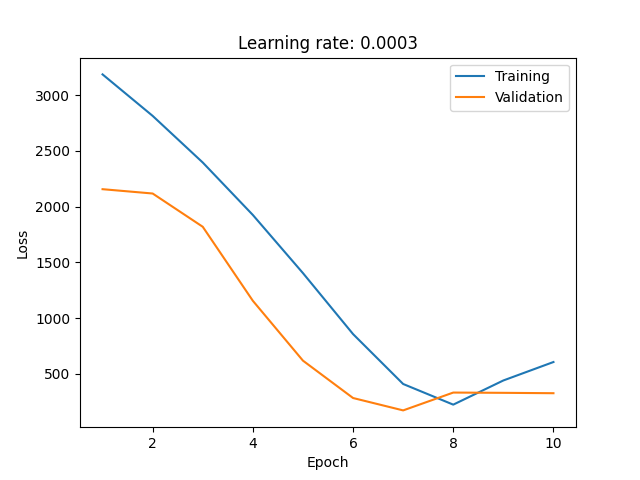
\includegraphics[width=\linewidth]{../outputs/age/age2/loss-curve.png}
        \caption{Age model learning curve on training and validation sets}
        \label{fig:age-learning-curve}
    \end{figure}

\subsubsection{Results}

    \begin{figure}[!htbp]
        \centering
        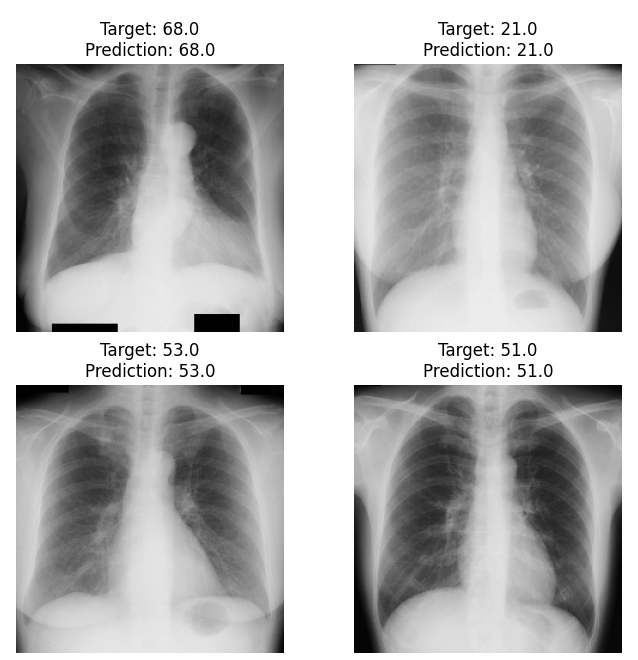
\includegraphics[width=\linewidth]{../outputs/age/age1/test-results-cropped.png}
        \caption{Age predictions on few samples of test data}
        \label{fig:age-results}
    \end{figure} 

    A total of 2 experiments were conducted with same hyperparameters and results are averaged. After fine-tuning the model, it was evaluated on the provided test samples on which it achieved a MAE of $5.57$ \Cref{fig:age-results} showcases some of the test samples along with their model predictions.
